\documentclass[10pt, conference, compsocconf]{IEEEtran}

\usepackage[margin=0.75in]{geometry}

\usepackage{amsfonts}
\usepackage{amssymb,amsmath}
\usepackage{hyperref}
\usepackage{algpseudocode}
\usepackage{graphicx}
%\usepackage{anyfontsize}   % for fontsize and selectfont command
\usepackage{array}         % better padding of cell content of tabulars
\usepackage[skip=2pt,font=footnotesize]{caption}

\usepackage{flushend}     % para usar flushend (no final)

\usepackage{tikz}       % for flowcharts
\usetikzlibrary{shapes, arrows}

\usepackage{times}

\newsavebox{\ieeealgbox}
\newenvironment{boxedalgorithmic}
  {\begin{lrbox}{\ieeealgbox}
   \begin{minipage}{\dimexpr\columnwidth-2\fboxsep-2\fboxrule}
   \begin{algorithmic}}
  {\end{algorithmic}
   \end{minipage}
   \end{lrbox}\noindent\fbox{\usebox{\ieeealgbox}}}

\newcommand{\scecore}{SCEcr }

\begin{document}

\title{ \vspace{0.25in}
A shuffled complex evolution algorithm for
the multidimensional knapsack problem using core concept}

\author{\IEEEauthorblockN{Marcos Daniel Valad\~ao Baroni}
\IEEEauthorblockA{ Departamento de Inform\'atica\\
Universidade Federal do Esp\'irito Santo\\
Vit\'oria, Esp\'irito Santo, Brazil\\
Email: mbaroni@ninfa.inf.ufes.br }
\and
\IEEEauthorblockN{Fl\'avio Miguel Varej\~ao}
\IEEEauthorblockA{ Departamento de Inform\'atica\\
Universidade Federal do Esp\'irito Santo\\
Vit\'oria, Esp\'irito Santo, Brazil\\
Email: fvarejao@ninfa.inf.ufes.br }
}

\maketitle

\begin{abstract}
This work addresses the application of a population based evolutionary algorithm
called shuffled complex evolution (SCE) in the core of multidimensional knapsack
problem (MKP).
The core of the MKP is a set of items which are hard to decide if they are or
not selected in good solutions.
This concept is used to reduce the original size of MKP instances.
%The SCE regards a natural evolution happening simultaneously in independent communities.
The performance of the SCE applied to the reduced MKP is verified through computational experiments
using well-known instances from literature.
The approach proved to be effective in finding near optimal solutions
demanding a small amount of processing time.
\end{abstract}
\IEEEpeerreviewmaketitle

\section{Introduction}
\label{sec:intro}

The multidimensional knapsack problem (MKP) is a strongly NP-hard combinatorial
optimization problem which can be viewed as a resource allocation problem and
defined as follows:

\begin{align}
  \text{maximize} & \sum_{j=1}^n p_j x_j \\
  \text{subject to} & \sum_{j=1}^n w_{ij} x_j \leqslant c_i \quad i \in \{1, \ldots, m\}\\
   & x_j \in \{0, 1\}, \quad j \in \{1, \ldots, n\}.
\end{align}

% Define the MKP
The problem can be interpreted as a set of $n$ items with profits $p_j$
and a set of $m$ resources with capacities $c_i$.
Each item $j$ consumes an amount $w_{ij}$ from each resource $i$, if selected.
The objective is to select a subset of items with maximum total profit,
not exceeding the defined resource capacities.
The decision variable $x_j$ indicates if $j$-th item is selected.
It is considered an integer programming problem (IP) since its variables $x_i$
are restricted to be integers.

The multidimensional knapsack problem can be applied on budget planning 
scenarios and project selections~\cite{mcmillan1973resource},
cutting stock problems~\cite{Gilmore-Gomory-1966}, loading problems~\cite{Shih-1979},
allocation of processors and databases in distributed computer programs~\cite{Gavish-Pirckul-1982}.

The problem is a generalization of the well-known knapsack problem (KP) in which
$m = 1$.
However it is a NP-hard problem significantly harder to solve in practice than the KP.
%Despite the existence of a fully polynomial approximation scheme (FPAS) for the KP,
%finding a FPAS for the MKP is NP-hard for $m \geqslant 2$~\cite{magazine1984note}.
Due its simple definition but challenging difficulty of solving, the MKP is often used to
to verify the efficiency of novel metaheuristics.

Its well known that the hardness of a NP-hard problem grows exponentially over
its size.
Thereupon, a suitable approach for tackling NP-hard problems is to reduce their size
through some variable fixing procedure.
Despite not guaranteeing optimality of the solution, an efficient variable
fixing procedure may provide near optimal solutions through a small computational effort.

%A metaheuristic is a set of concepts that can be used to define heuristic methods
%that can be applied to a wide set of different problems.
%In other words, a metaheuristic can be seen as a general algorithmic framework which can be applied to
%different optimization problems with relatively few modifications to make them adapted to a specific problem.”

The SCE is a metaheuristic proposed by Duan in \cite{duan1992effective}
which combines the ideas of a controlled random search with the concepts
of competitive evolution and shuffling.
The SCE algorithm has been successfully used to solve several problems
like flow shop scheduling~\cite{zhao2014shuffled}, project management~\cite{elbeltagi2007modified}
and MKP~\cite{baroni2015shuffled}.

This work addresses the development of an hybrid heuristic using an
efficient variable fixing procedure and the SCE metaheuristic, as an improvement
proposal for the work in \cite{baroni2015shuffled}

The reminder of the paper is organized as follows:
Section~\ref{sec:core} defines the core concept for the MKP and its application
in the problem reduction.
Section~\ref{sec:sce} presents the shuffled complex evolution algorithm
and proposes its application on the MKP.
Section~\ref{sec:exp} comprises several computational experiments over well-known
instances from literature.
In section~\ref{sec:conc} we make our concluding remarks about the developed
methods and the experimental results.



\section{The core concept for MKP}
\label{sec:core}
The core concept was first presented for the one-dimensional 0-1 knapsack problem (KP),
leading to very successful KP algorithms.
The main idea is to reduce the original problem by only considering a set of
items for which it is hard to decide if they will occur or not in an optimal solution.
This set of items is named core.
The variables for all items outside the core are fixed to certain values.

The knapsack problem considers items $j = 1, \ldots, n$, associated profits $p_j$ and
associated weights $w_j$.
A subset of these items has to be selected and packed into a knapsack having capacity $c$.
The total profit of the items in the knapsack has to be maximized, while the
total weight is not allowed to exceed $c$.

Before defining the core of the KP it is worth to note the solution structure
of its LP-relaxation.
The LP-relaxation of an integer programming problem arises by replacing the
constraint that each variable must be integer by a constraint that allows
continuity of the variable.
The LP-relaxation of a KP is found by replacing the constraint $x_i \in \{0,1\}$
by $0 \leqslant x_i \leqslant 1$ for all $i \in \{1, \ldots, n\}$.
If the items are sorted according to decreasing efficiency values
\begin{displaymath}
  e_j = \frac{p_j}{w_j},
\end{displaymath}
it is known that the solution of the LP-relaxation consists of
three consecutive parts: the first part contains variables set to $1$, the second
pare consists of at most one split item $s$, whose corresponding LP-values is
fractional, and finally the remaining variables, which are always set to zero,
form the third part.

For most instance of KP (except those with a very special structure) the integer
optimal solution closely corresponds to this partitioning in the sense that it
contains most of the highly efficient items of the first part, some items with
medium efficiencies near the split item, and almost no items with low efficiencies
from the third part.
Items of medium efficiency constitute the core.

Balas and Zemel~\cite{balas1980algorithm} gave the following precise definition
of the core of a KP, based on the knowledge of an optimal integer solution $x^*$.
Assume that the items are sorted according to decreasing efficiencies and let
\begin{displaymath}
  a := \min\{ j | x_j^* = 0 |\}, \quad b := \max\{ j | x_j^* = 1 \}.
\end{displaymath}
The core is given by the items in the interval $C = \{a, \ldots, b\}$.
It is obvious that the split item is always part of the core, i.e., $a < s < b$.

Figure~\ref{fig:kpecore} illustrates an exact core for an hypothetical KP instance
with $13$ items.
First row represents the efficiency value $e$ of each item.
The items are sorted by descending order of efficiency.
Second row represent solution array of the LP-relaxation.
The third row represents the exact solution for the original problem.
The $8$-th item is the split item.
Notice that the split item is within the exact core.

\begin{figure}[h]
  \centering
  \includegraphics[scale=0.406]{imgs/core}
  \caption{Example of exact core for a hypothetical KP instance.}
  \label{fig:kpecore}
\end{figure}

The KP Core problem (KPC) is defined as
\begin{align*}
  \text{maximize} & \sum_{j \in C} p_j x_j  + \tilde{p}\\
  \text{subject to} & \sum_{j \in C} w_{j} x_j \leqslant c - \tilde{w}\\
  & x_j \in \{0, 1\}, \quad j \in C.
\end{align*}
with $\tilde{p} = \sum^{a-1}_{j=1} p_j$ and $\tilde{w} = \sum^{a-1}_{j=1} w_j$
respectively quantifying the total profit and the total weights of items fixed as selected.
The solution of KPC would suffice to compute the optimal solution of KP, which
however, has to be already partially known to determine $C$.
Nevertheless an approximate core $C = \{s-\delta, \ldots, s+\delta\}$,
of fixed size $|C| = 2\delta+1$ is considered for a heuristic reduction of the problem.

Figure~\ref{fig:kpcore} exemplifies an approximate core of a hypothetical KP
instance with $13$ items.
The first row represents the efficiency value of each item and the second row
represents the value of each variable on the LP-relaxation optimal solution.
The items are sorted in descending order of efficiency value.
The last row illustrates the variable fixing after the defined core.
Asterisks indicate free variables associated to the items in the
approximate core.

\begin{figure}[h]
  \centering
  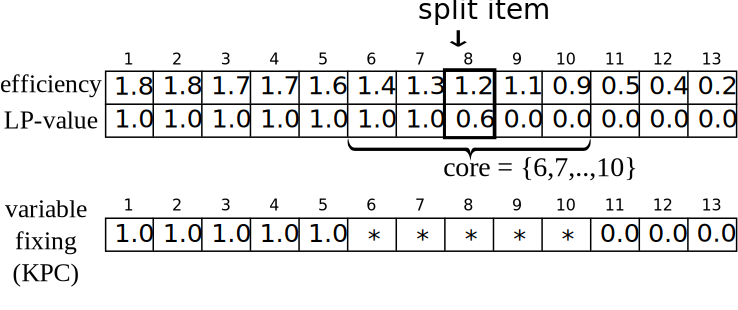
\includegraphics[scale=0.406]{imgs/kp_3}
  \caption{Example of core for a hypothetical KP instance with $n=13$ and approximate core size of $5$ ($\delta = 2$).}
  \label{fig:kpcore}
\end{figure}

\subsection{The Core Concept for MKP}

The previous definition of the core for KP can be extended to MKP without major
difficulties, once an efficiency measure is defined for the MKP,
as addressed in \cite{puchinger2006core}, even though,
a proper efficiency measure for MKP is not obvious due the
multidimensional weight of the items.
A well accepted efficiency measure is discussed in Section~\ref{subsec:dual}.

Now let $x^*$ be an optimal solution for a MKP and assume that the items are
sorted in descending order after some given efficiency measure. Then let
\begin{displaymath}
  a = \min \{ j | x_j^* = 0 \}, \quad b = \max \{ j | x_j^* = 1 \}.
\end{displaymath}
The core is given by the items in the interval $C = \{ a, \ldots, b \}$,
and the multidimensional knapsack core problem (MKPC) defined as
\begin{align*}
  \text{maximize} & \sum_{j \in C} p_j x_j  + \tilde{p}\\
  \text{subject to} & \sum_{j \in C} w_{ij} x_j \leqslant c_i - \tilde{w}_i, \quad i = 1, \ldots, m\\
  & x_j \in \{0, 1\}, \quad j \in C.
\end{align*}
with $\tilde{p} = \sum^{a-1}_{j=1} p_j$  and $\tilde{w}_i = \sum^{a-1}_{j=1} w_{ij}, i = 1, \ldots, m$.

In contrast to KP, the solution of the LP-relaxation of MKP in general does not
consists of a single fractional split item. But up to $m$ fractional values give
rise to a whole \emph{split interval} $S = \{ s_1, \ldots, s_m\}$, where
$s_1$ and $s_m$ are respectively the first and the last index of variables with
fractional values after sorting by the given efficiency measure.
Once the split interval is defined, a central index value $s = \lfloor \frac{s_1+s_m}{2}\rfloor$
can be used as the center of an approximate core.

\subsection{The Dual-variable Efficiency Measure}
\label{subsec:dual}
For defining a reasonable efficiency measure for MKP consider the most obvious
form of efficiency which is a direct generalization of the one-dimensional case:
\begin{displaymath}
	e_j(simple) = \frac{p_j}{\sum_{i=1}^{m} w_{ij}}
\end{displaymath}
In this definition different orders of magnitude of the constraints are not
considered and a single constraint may dominate the others.
This drawback can be avoided by introducing relevance values $r_i$ for every
constraint:
\begin{displaymath}
	e_j(relevance) = \frac{p_j}{\sum_{i=1}^{m} r_i w_{ij}}
\end{displaymath}
Several proposals for setting the relevance values $r_i$ were discussed and
tested by Puchinger, Raidl and Pferschy in \cite{puchinger2006core}.
According to their work setting the relevance values $r_i$ to the values of an
optimal solution to the dual problem of the MKP's LP-relaxation, as suggested
in \cite{Chu-Beasley-1998}, achieved the best results and will be the one
considered in this work for the development of the hybrid heuristic.

While the original MKP can be seen as a resource allocation problem,
the dual problem of the MKP can be seen as a resource valuation problem.
For this reason the values of the dual solution is related to the
\emph{importance} of each resource.

The split interval resulting from the efficient measure considered can be
precisely characterized.
Let $x^{LP}$ be the optimal solution of the LP-relaxation of MKP.
Then the following relation holds, as proved in \cite{puchinger2006core}:
\begin{displaymath}
 x_l^{LP} =
  \begin{cases}
    1         & \mbox{if } e_j > 1, \\
    \in [0,1] & \mbox{if } e_j = 1, \\
    0         & \mbox{if } e_j < 1.
  \end{cases}
\end{displaymath}
From this relation we can note that all variables in the split interval will
have efficiency measure $e_j = 1$, while less and more efficient ones will have
$e_j < 1$ and $e_j > 1$ respectively.

Figure~\ref{fig:mkpcore} exemplifies an approximate core of a hypothetical MKP
with $13$ variables and $3$ dimensions.
Notice that the LP-relaxation solution has now $3$ fractional variables that
defines the center of the split interval.

\begin{figure}[h]
  \centering
  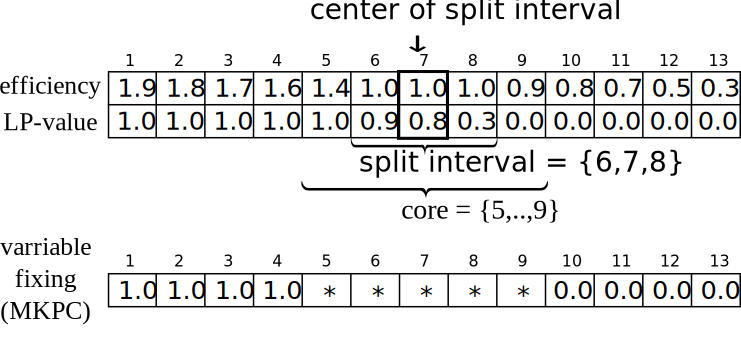
\includegraphics[scale=0.406]{imgs/mkp_3}
  \caption{Example of core for a hypothetical MKP instance with $n=13$, $m=3$ and approximate core size of $5$ ($\delta = 2$).}
  \label{fig:mkpcore}
\end{figure}

The following section presents the shuffled complex evolution algorithm
and proposes its application on the MKP.


\section{The shuffled complex evolution for the MKP}
\label{sec:sce}
The {\bf shuffled complex evolution} (SCE) \cite{duan1992effective}
is a population
based evolutionary optimization algorithm that regards a natural 
evolution happening simultaneously in $N$ independent communities (or {\bf complexes}).

Initialy $N*M$ individuals are randomly taken from the feasible solution space and
sorted according to their fitness.
Subsequently a {\bf shuffling} process places the \nth{1} in the first complex,
the \nth{2} in second complex, individual N\ts{th} goes to N\ts{th} complex,
individual $M+1$ goes back to the first complex, etc.
\vspace*{-20pt}
\begin{center}
\noindent\begin{tabular}{@{\hspace{0.0em}}c@{\hspace{1.0em}}c@{\hspace{0.0em}}}
\hspace{-3mm}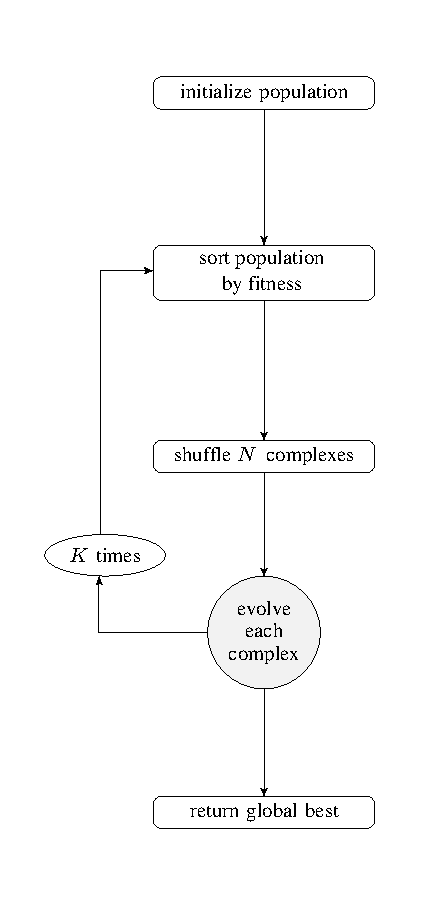
\includegraphics[width=0.46\linewidth]{imgs/flow1a} &
\hspace{-3mm}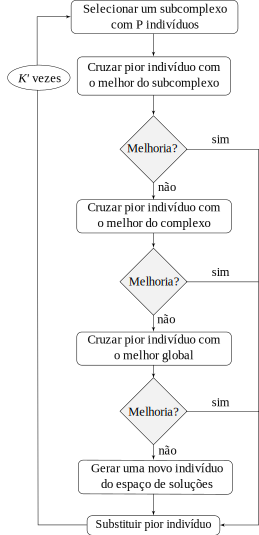
\includegraphics[width=0.46\linewidth]{imgs/flow2} \\
{\scriptsize The SCE algorithm.} & {\scriptsize Evolving stage.}
\end{tabular}
\end{center}
The next step after shuffling the complexes is to evolve each each of then through
a fixed amount of {\it (a)} $K'$ steps.
In each step {\it (b)} a {\bf subcomplex} of $P$ individuals is selected from the
complex, prioritizing those with better fitness.

The worst individual from the  subcomplex is identified to
be replaced by a new one generated by {\it (c)} its crossing 
with best individual of the subcomplex.

If the new solution has not improved {\it (d)} the best individual
of the {\bf complex} is considered for crossing and latter the {\it (e)} best one  
of whole {\bf population}.
If all the crossing steps couldn't improve the worst individual,
it is {\it (f)} replaced by a {\bf new random} solution.


\section{Computational experiments}
\label{sec:exp}
To verify the efficiency of the proposed hybrid metaheuristic, several computational
experiments was executed considering the original SCE for the MKP proposed in
\cite{baroni2015shuffled} and the hybrid SCE, proposed in this work.
For brevity the hybrid SCE proposed in this work will be referred to as \scecore.

For the experiments, two sets of MKP instances was used:
a first set composed by 270 instances provided by Chu and Beasley (\cite{Chu-Beasley-1998})
and a second set composed by 11 instances provided by Glover and Kochenberger in
\cite{glover1996critical}.
These instances are all available at \cite{ORLibrary}.
%Afterwards two main tests was considered:
%(a) using the well-known set of problems defined by Chu and Beasley (\cite{Chu-Beasley-1998})
%and (b) a large set of randomly generated instances using uniform distribution.

The set of MKP instances provided by Chu and Beasley was generated using a
procedure suggested by Freville and Plateau~\cite{freville1994efficient}, which
attempts to generate instances hard to solve.
The number of constraints $m$ varies among $5$, $10$ and $30$, and the number
of variables $n$ varies among $100$, $250$ and $500$.

The $w_{ij}$ were integer numbers drawn from the discrete uniform distribution
$U(0, 1000)$.
The capacity coefficient $c_i$ were set using
$b_i = \alpha\sum_{j=1}^{n} w_{ij}$ where $\alpha$ is a tightness ratio and
varies among $0.25$, $0.5$ and $0.75$.
For each combination of $(m,n,\alpha)$ parameters, $10$ random problems was generated,
totaling $270$ problems.
The profit $p_j$ of the items were correlated to $w_{ij}$ and generated as follows:
\begin{displaymath}
  p_j = \sum_{i=1}^m \frac{w_{ij}}{m} + 500q_j \qquad j = 1, \ldots, n
\end{displaymath}

%\subsection{The set of random instances}

%The second set of instances is composed by problems generated using a similar
%setup.
%The only differences is that the profit $p_j$ is also drawn from a discrete uniform
%distribution $U(0, 1000)$.
%For each combination of $(m, n, \alpha)$ parameter, $600$ random problems was
%generated, totaling $16200$ problems.

\subsection{Experimental results}

All the experiments were run on a Intel$^R$ Core i5-3570 CPU @3.40GHz computer
with 4GB of RAM.
The original SCE and \scecore was both implemented in C programming language.
%For the set of random instance all best known solution was found by the solver
%SCIP 3.0.1 running for at least 10 minutes.

For the variable fixing procedure used on \scecore, the range size of the approximate core was
$|C| = m+\frac{n}{10}$ for all instances.
In all instances the parameters used for SCE and \scecore were the same recommended
in \cite{baroni2015shuffled} which was found after a batch test using Chu and Beasley instances:
\begin{itemize}
  \item $N = 20$: number of complexes;
  \item $M = 20$: number of individuals in each complex;
  \item $P = 5$: number of individuals in each subcomplex;
  \item $K = 300$: number of algorithm iterations;
  \item $K' = 20$: number of iterations used in the complex evolving process;
  \item $c = n/5$: number of genes carried from parent in crossing process.
\end{itemize}

Table~\ref{tab:chu} shows the performance of the SCE and \scecore on the Chu-Beasley set of instances.
Each instance in the set was executed 10 times for each algorithm.
Columns \textit{n}, \textit{m} and \textit{$\alpha$} shows the parameters used
on each instance generation.
The \textit{time} column shows the average execution time of the algorithms (lower is better).
The \textit{quality} column shows the average ratio of the solution found and
the best known solution from literature (\cite{vimont2008reduced, della2012improved}) of each instance (higher is better).

It can be observed that the \scecore had faster convergence speed, achieving higher
quality solutions in all cases, achieving at least $99.02\%$ of best known, in less than $2$ seconds
for every instance.

It can be also noticed that \scecore executed in much less processing time than original
SCE.
This is due the variable fixing procedure which reduced the problem size,
resulting in less genes operations during the evolving procedures.
The variable fixing procedure also brought robustness for the method, as the quality
of the solution found increased in case of larger instances while on original
SCE the quality decreased considerably.

\begin{table}
{
\renewcommand{\arraystretch}{1.3}%
\fontsize{8.5pt}{1em}\selectfont 
\begin{center}
  \begin{tabular}{|r|r|r|rr|rr|} \cline{4-7}
  \multicolumn{3}{c|}{} &  \multicolumn{2}{c|}{\bf time (s)} & \multicolumn{2}{c|}{\bf quality (\%)} \\ \hline
\textbf{n}   & \textbf{m}  & \textbf{$\alpha$} &
  \textbf{SCE} & \textbf{\scecore} & {\bf SCE} & {\bf \scecore}  \\ \hline
100 &  5 & 0.25 & 0.79 & 0.15 & 96.5 & 99.73 \\
    &    & 0.50 & 0.81 & 0.15 & 97.4 & 99.86 \\
    &    & 0.75 & 0.83 & 0.13 & 98.9 & 99.91 \\ \cline{2-7}
    & 10 & 0.25 & 0.75 & 0.22 & 95.7 & 99.53 \\
    &    & 0.50 & 0.93 & 0.22 & 96.7 & 99.76 \\
    &    & 0.75 & 0.89 & 0.22 & 98.5 & 99.96 \\ \cline{2-7}
    & 30 & 0.25 & 1.01 & 1.00 & 95.4 & 99.02 \\
    &    & 0.50 & 1.07 & 0.79 & 96.4 & 99.21 \\
    &    & 0.75 & 0.99 & 0.77 & 98.2 & 99.52 \\ \cline{2-7}
    & \multicolumn{2}{r|}{\textbf{average}}  & 0.90 & {\bf 0.41} & 97.5 & {\bf 99.50} \\ \hline
250 &  5 & 0.25 & 1.72 & 0.54 & 93.2 & 99.87 \\
    &    & 0.50 & 1.75 & 0.55 & 94.9 & 99.94 \\
    &    & 0.75 & 1.78 & 0.51 & 97.6 & 99.95 \\ \cline{2-7}
    & 10 & 0.25 & 1.84 & 0.67 & 93.1 & 99.57 \\
    &    & 0.50 & 1.84 & 0.62 & 94.6 & 99.80 \\
    &    & 0.75 & 1.81 & 0.64 & 97.2 & 99.88 \\ \cline{2-7}
    & 30 & 0.25 & 2.21 & 1.16 & 93.2 & 99.46 \\
    &    & 0.50 & 2.21 & 0.96 & 94.2 & 99.36 \\
    &    & 0.75 & 2.31 & 1.03 & 96.6 & 99.59 \\ \cline{2-7}
    & \multicolumn{2}{r|}{\textbf{average}} & 1.94 & {\bf 0.74} & 95.0 & {\bf 99.60} \\ \hline
500 &  5 & 0.25 & 3.16 & 0.85 & 91.4 & 99.77 \\
    &    & 0.50 & 3.18 & 0.86 & 93.4 & 99.87 \\
    &    & 0.75 & 3.34 & 0.84 & 96.4 & 99.92 \\ \cline{2-7}
    & 10 & 0.25 & 3.39 & 0.99 & 91.7 & 99.49 \\
    &    & 0.50 & 3.37 & 0.97 & 93.1 & 99.78 \\
    &    & 0.75 & 3.44 & 0.95 & 96.2 & 99.83 \\ \cline{2-7}
    & 30 & 0.25 & 3.83 & 1.53 & 91.4 & 99.75 \\
    &    & 0.50 & 3.90 & 1.48 & 92.6 & 99.42 \\
    &    & 0.75 & 3.99 & 1.42 & 96.0 & 99.68 \\ \cline{2-7}
    & \multicolumn{2}{r|}{\textbf{average}} & 3.51 & {\bf 1.10} & 93.58 & {\bf 99.61} \\ \hline
\end{tabular}

\end{center}
}
 \caption{SCE and \scecore  performance on Chu-Beasley problems.}
 \label{tab:chu}
\end{table}

Table~\ref{tab:gk} shows the performance of \scecore on the Glover-Kochenberger set of instances.
Each instance in the set was executed 10 times.
Columns \textit{n} and \textit{m} indicate the size of each instance.
The \textit{SCEcr time} column shows the average execution time of SCEcr algorithm.
The \textit{quality} column shows the average ratio of the solution found by \scecore and
the best known solution of each instance.
It can be noticed that SCEcr achieved high quality solutions, at least $99.10\%$
of best known solution, spending very small amount of processing time, compared
to the time taken to find the best known solutions.

\begin{table}
{
\renewcommand{\arraystretch}{1.7}%
\fontsize{8.5pt}{1em}\selectfont 
\begin{center}
\begin{tabular}{|r|r|r|r|r|} \hline
		\textbf{\#} & \textbf{n}   & \textbf{m}  & \textbf{SCEcr time (s)} & \textbf{quality (\%)} \\ \hline
01 & 100 & 15 & 0.31 & 99.68 \\ \hline
02 & 100 & 25 & 0.47 & 99.51 \\ \hline
03 & 150 & 25 & 0.79 & 99.60 \\ \hline
04 & 150 & 50 & 1.61 & 99.10 \\ \hline
05 & 200 & 25 & 0.83 & 99.73 \\ \hline
06 & 200 & 50 & 1.67 & 99.30 \\ \hline
07 & 500 & 25 & 1.27 & 99.72 \\ \hline
08 & 500 & 50 & 2.06 & 99.62 \\ \hline
09 &1500 & 25 & 1.83 & 99.32 \\ \hline
10 &1500 & 50 & 5.25 & 99.76 \\ \hline
11 &2500 &100 &11.94 & 99.77 \\ \cline{1-5}
    \multicolumn{4}{|r|}{\textbf{average quality}}  & $\bf 99.46$  \\ \hline
\end{tabular}
\end{center}
}
 \caption{\scecore performance on Glover-Kochenberger problems.}
 \label{tab:gk}
\end{table}

%\begin{table}
%{
%\renewcommand{\arraystretch}{1.5}%
%\fontsize{8.5pt}{1em}\selectfont 
%\begin{center}
%\begin{tabular}[c]{|r|r|r|rrr|} \hline
%\textbf{n}   & \textbf{m}  & \textbf{$\alpha$}    &\textbf{SCIP time (s)}& \textbf{SCE time (s)} & \textbf{gap (\%)} \\ \hline
%100 &  5 & 0.25 & $  0.93$ & $  0.41$  & $98.3$ \\
%    &    & 0.50 & $  0.28$ & $  0.39$  & $99.3$ \\
%    &    & 0.75 & $  0.09$ & $  0.37$  & $99.8$ \\ \cline{2-6}
%    & 10 & 0.25 & $  3.15$ & $  0.41$  & $98.2$ \\
%    &    & 0.50 & $  0.71$ & $  0.40$  & $99.3$ \\
%    &    & 0.75 & $  0.16$ & $  0.37$  & $99.8$ \\ \cline{2-6}
%    & 30 & 0.25 & $  7.26$ & $  0.42$  & $98.3$ \\
%    &    & 0.50 & $  1.47$ & $  0.42$  & $99.3$ \\
%    &    & 0.75 & $  0.25$ & $  0.38$  & $99.8$ \\ \cline{2-6}
%    & \multicolumn{4}{r}{\textbf{average gap}}  & $\bf 99.1$  \\ \hline \hline
%\textbf{n}   & \textbf{m}  & \textbf{$\alpha$}    &\textbf{SCIP time (s)}& \textbf{SCE time (s)} & \textbf{gap (\%)} \\ \hline
%250 &  5 & 0.25 & $ 58.20$ & $  1.10$  & $97.2$ \\
%    &    & 0.50 & $  8.51$ & $  1.04$  & $98.9$ \\
%    &    & 0.75 & $  0.51$ & $  0.90$  & $99.7$ \\ \cline{2-6}
%    & 10 & 0.25 & $227.94$ & $  1.11$  & $97.6$ \\
%    &    & 0.50 & $ 43.69$ & $  1.02$  & $99.0$ \\
%    &    & 0.75 & $  1.59$ & $  0.90$  & $99.8$ \\ \cline{2-6}
%    & 30 & 0.25 & $270.48$ & $  1.20$  & $97.7$ \\
%    &    & 0.50 & $ 88.73$ & $  1.09$  & $99.0$ \\
%    &    & 0.75 & $  2.90$ & $  0.94$  & $99.8$ \\ \cline{2-6}
%    & \multicolumn{4}{r}{\textbf{average gap}}  & $\bf 98.7$  \\ \hline \hline
%\textbf{n}   & \textbf{m}  & \textbf{$\alpha$}    &\textbf{SCIP time (s)}& \textbf{SCE time (s)} & \textbf{gap (\%)} \\ \hline
%500 &  5 & 0.25 & $278.85$ & $  2.23$  & $96.1$ \\
%    &    & 0.50 & $177.32$ & $  2.14$  & $98.4$ \\
%    &    & 0.75 & $  8.47$ & $  1.87$  & $99.6$ \\ \cline{2-6}
%    & 10 & 0.25 & $284.11$ & $  2.30$  & $96.7$ \\
%    &    & 0.50 & $275.68$ & $  2.16$  & $98.6$ \\
%    &    & 0.75 & $ 33.67$ & $  1.90$  & $99.7$ \\ \cline{2-6}
%    & 30 & 0.25 & $283.78$ & $  2.50$  & $96.9$ \\
%    &    & 0.50 & $283.54$ & $  2.32$  & $98.7$ \\
%    &    & 0.75 & $ 71.66$ & $  1.96$  & $99.7$ \\ \cline{2-6}
%    & \multicolumn{4}{r}{\textbf{average gap}}  & $\bf 98.3$  \\ \hline
%\end{tabular}
%\end{center}
%}
% \caption{SCE performance on the random generated problems.}
% \label{tab:rand}
%\end{table}

%\begin{figure}
%  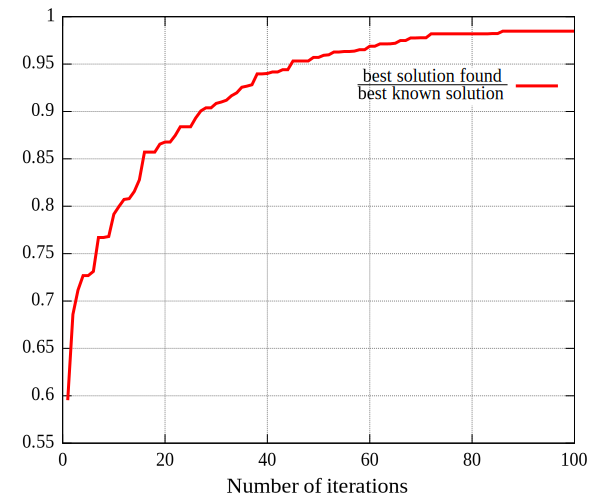
\includegraphics[scale=0.5]{imgs/iter}
%  \caption{Convergence process of SCE for MKP
%    for a problem with $n=500$, $m=30$ and $t=0.50$.}
%  \label{fig:iter}
%\end{figure}

%The fast convergence speed of SCE for MKP can be noticed in Fig.~\ref{fig:iter}.
%The figure shows for each iterations step, the quality of best solution found
%for the first $100$ iterations.
%The problem instance used was taken from the second set of problem (random instances).
%The best known solution was found with $600$s of execution on SCIP solver and
%the execution of the SCE algorithm expended $1.1$ seconds.


\section{Conclusions and future remarks}
\label{sec:conc}

In this paper we addressed the development of a hybrid heuristic for the MKP
implementing a population based algorithm called shuffled complex evolution
for solving the multidimensional knapsack problem assisted by an efficient
variable fixing procedure.
Its performance was verified through several computational experiments.

The SCE algorithm, which combines the ideas of a controlled random search with
the concepts of competitive evolution, proved to be able to achieve fast
convergence ratio, finding good quality near optimal solutions, demanding small
amount of computational time.

The application of the core concept, through a variable fixing procedure for MKP,
proved to be efficient to reduce the size of the problems which provided fast
execution time, producing higher quality solutions.

\scecore algorithm presented faster convergence speed, achieving higher
quality solutions in all cases, achieving at least $99.02\%$ of best known, in less than $2$ seconds
for every instance.
The variable fixing procedure also brought robustness for the method, as the quality
of the solution found increased in case of larger instances.

The hybrid heuristic developed in this papter is very well suitable if it is necessary
to compute a good solution in a small processing time.
The hybrid heuristic could achieved $99.61\%$ on average of quality of the best known solution for
the 270 Chu-Beasley instances and $99.46\%$ on average for the Glover-Kochenberger instances.

Future works include the investigation of different crossing procedures 
and the use of local search in the process of evolving complexes.
Besides we want to investigate the possibility of using the efficiency measure
concept directly on metaheuristics.



%\newpage

%\bibliographystyle{abbrv}
\bibliographystyle{IEEEtran}
\bibliography{../../../refs}

%\printbibliography
\flushend

\end{document}

